\documentclass[10pt,twocolumn,letterpaper]{article}


\usepackage{times}
\usepackage{epsfig}
\usepackage{graphicx}
\usepackage{amsmath}
\usepackage{amssymb}

% Include other packages here, before hyperref.

% If you comment hyperref and then uncomment it, you should delete
% egpaper.aux before re-running latex.  (Or just hit 'q' on the first latex
% run, let it finish, and you should be clear).
\usepackage[breaklinks=true,bookmarks=false]{hyperref}


% Pages are numbered in submission mode, and unnumbered in camera-ready
%\ifcvprfinal\pagestyle{empty}\fi
\setcounter{page}{1}
\begin{document}

%%%%%%%%% TITLE
\title{CMPT459 Data Mining\\
Milestone1}


\author{Ziyi An\\
301371687\\
% For a paper whose authors are all at the same institution,
% omit the following lines up until the closing ``}''.
% Additional authors and addresses can be added with ``\and'',
% just like the second author.
% To save space, use either the email address or home page, not both
\and
Chen Zhao\\
301308092\\

\and

Duo Lu\\
301368672
}


\maketitle
%\thispagestyle{empty}



%-------------------------------------------------------------------------



%------------------------------------------------------------------------


%%%%%%%%% BODY TEXT
\section{Introduction}
This is the report for the data mining project, phase one, which is majorly exploring data preprocess procedure, as well as some visualization of the raw data. The results for the first submissions are discussed in the following paragraphs, and the necessary code to produce those conclusions are within the Git repository, along with some extra experiments (involving visualization and feature extraction) which are, we think, beneficial to the project. Some technical details are also demonstrated in the README file.


\section{Exploratory Data Analysis}
This section is incrementally improved by the 2nd step as suggested. 

\-

1. The histograms of price before and after cleaning is as follows:   

\begin{figure}[h!]%
    \centering
    \subfloat{{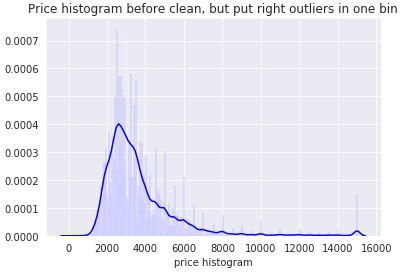
\includegraphics[width=3.2cm]{CMPT459_1.png} }}%
    \qquad
    \subfloat{{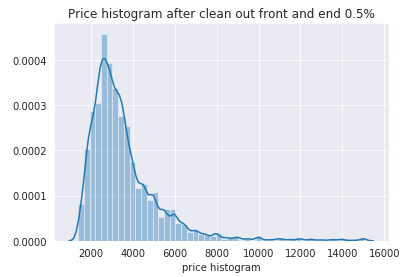
\includegraphics[width=3.22cm]{CMPT459_2.png} }}%
    \caption{}%
    \label{fig:example}%
\end{figure}

For the values of latitude and longitude, intuitively, we rule out some points according to the geographical information of NYC, and then plot the histograms as follows. Those “outliers” will be discussed in the next section.

\begin{figure}[h!]%
    \centering
    \subfloat{{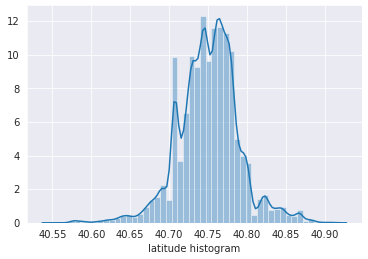
\includegraphics[width=3.2cm]{CMPT459_3.png} }}%
    \qquad
    \subfloat{{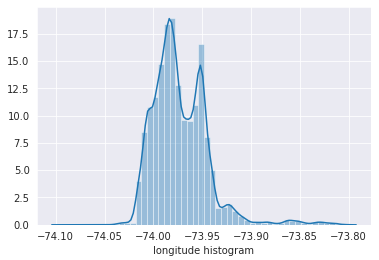
\includegraphics[width=3.22cm]{CMPT459_4.png} }}%
    \caption{}%
    \label{fig:example}%
\end{figure}


2. The hour-wise listing trend is illustrated in histogram as well, and the top 5 are obtained by code (or eyeball).
\\
\begin{figure}[h!]
    \centering
    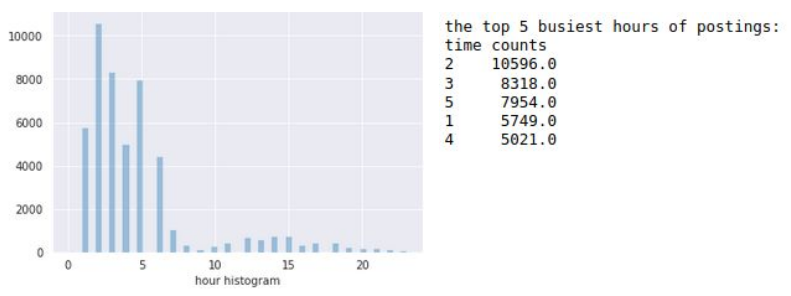
\includegraphics[width=7cm]{CMPT459_Pair1.png}
    \caption{}
    \label{fig:galaxy}
\end{figure}

\clearpage

3. The proportion of target variable values (interest level) is represented in both pie chart and bar plot as follows:



\begin{figure}[h!]
    \centering
    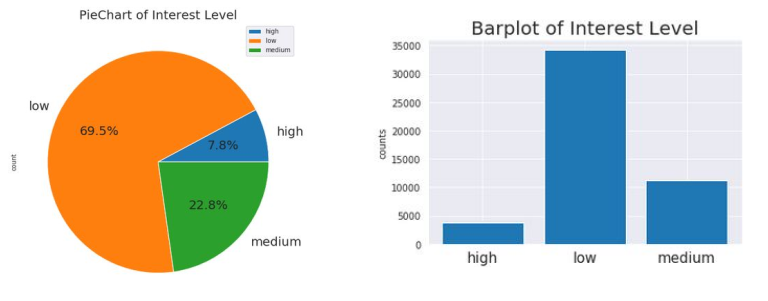
\includegraphics[width=7cm]{CMPT459_pair2.png}
    \caption{}
    \label{fig:galaxy}
\end{figure}


*4. In addition to the required procedures, some other visualizations that might be helpful are produced, such as the statistical summaries and histograms of price in each interest level:  


\begin{figure}[h!]%
    \centering
    \subfloat{{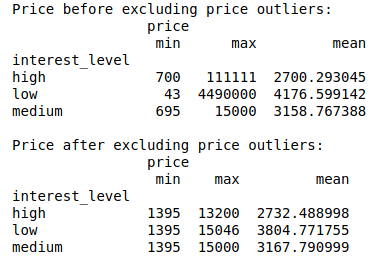
\includegraphics[width=3.2cm]{CMPT459_7.png} }}%
    \qquad
    \subfloat{{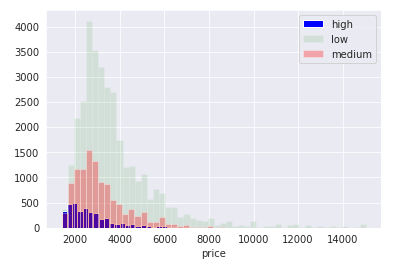
\includegraphics[width=3.22cm]{CMPT459_8.png} }}%
    \caption{}%
    \label{fig:example}%
\end{figure}


We also use google map API to label each rental on a map of NYC according to the lat/longitudes. The following is the output of a 10\% random sample from the original data. 


\begin{figure}[h!]
    \centering
    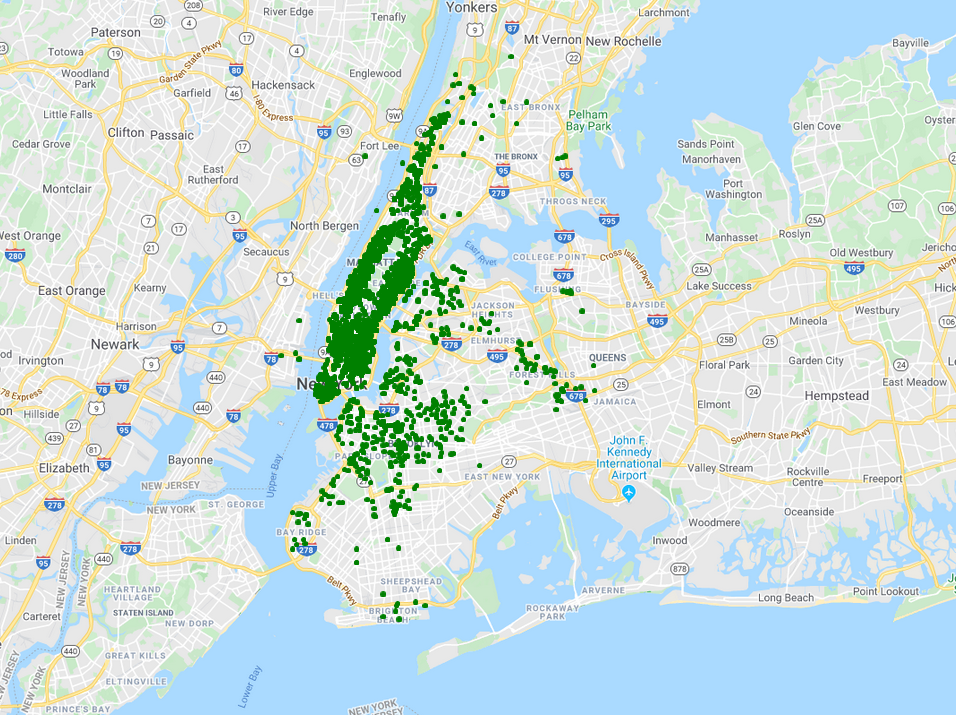
\includegraphics[width=7cm]{rents_sample.png}
    \caption{Note that the API key is not uploaded to the git repo}
    \label{fig:galaxy}
\end{figure}


%-------------------------------------------------------------------------



%------------------------------------------------------------------------S



\section{Dealing with missing values, outliers}

1. A short summary of missing values in each variable is as such:


\begin{figure}[h!]
    \centering
    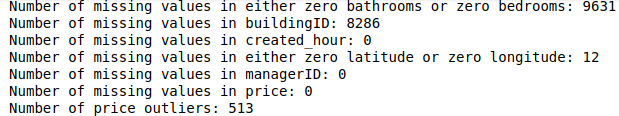
\includegraphics[width=7cm]{CMPT459_9.png}
    \caption{}
    \label{fig:galaxy}
\end{figure}

They are detected by values like 0, None, empty string, empty list, etc. Other missing values in text (ie, feature, address, description) would be further processed in the next section so that they could be decided to drop or not.

\-

2.Variables that are capable of having outliers are Price, Latitude & Longitude. They can either be defined manually by some bonding a percentile, geographical information (0.5\% each end, NYC coordinates) or automatically by statistical measurements (Z-scores). The output of the latter approach is partially as follows: 


\begin{figure}[h!]
    \centering
    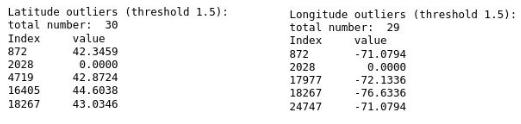
\includegraphics[width=7cm]{CMPT459_pair3.png}
    \caption{}
    \label{fig:galaxy}
\end{figure}


\begin{figure}[h!]
    \centering
    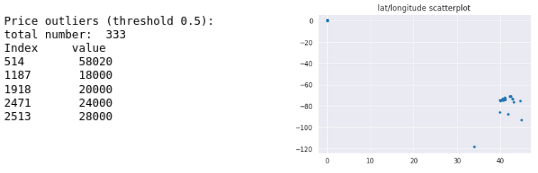
\includegraphics[width=7cm]{CMPT459_pair4.png}
    \caption{}
    \label{fig:galaxy}
\end{figure}


The boxplot of each variable is quite influenced by the remote outliers, and the price histogram of uncleaned data has been shown in the previous section, which indicates outliers. A scatter plot of lat&longitude together might be a way of addressing the outliers as above. 




3.About the outliers and the missing values, if we are really rigorous to dealing rental information of NYC (only), empirically, some coordinates are considered to be noises and should be removed, while the missing values could be computed according to the address information. (We were trying this idea until realizing that there might be a payment of the Google API involved. ) The outliers of prices are considered to be deleted as, empirically, some values are quite unreasonable to be a rental price (, a selling price rather). Therefore, they should be detected (according to some threshold subjective to define) and removed. 
Other variables either have no missing value, like managerID and created hour, or should not be defined as missing, like zeros in bath/bedroom . Anyhow, most records would not be removed except maybe the price outliers as they intuitively would influence the trained classifier, and they are difficult to be inferred by other information.




%-------------------------------------------------------------------------



%------------------------------------------------------------------------S



\section{Feature Extraction from Images and Text}
1.The image feature extraction is troublesome since the total data amount is too massive to be either downloaded as a whole or individually  loaded as the program goes. Primarily, we have easily computed the number images (URLs) in each record as a feature. Moreover, we have tried to extract the logo information from each image as one of the extra code file has shown. The major problem encountered was the running time (using CSIL computers) that we hope to resolve later.



\begin{figure}[h!]%
    \centering
    \subfloat{{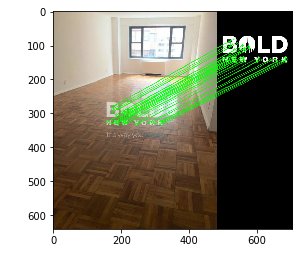
\includegraphics[width=3.2cm]{Screenshot from 2020-02-05 22-40-36.png} }}%
    \qquad
    \subfloat{{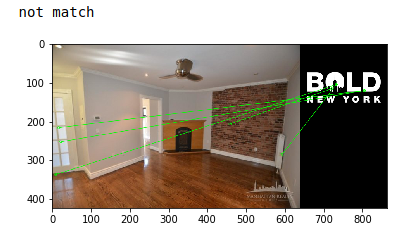
\includegraphics[width=3.22cm]{Screenshot from 2020-02-05 22-41-15.png} }}%
    \caption{}%
    \label{fig:example}%
\end{figure}


2. The columns ‘features’ and 'description' are what we mainly focused text information extraction. We build pipelines to formally conduct the work for both features and description. 
\\ For 'Features' (Figure 11):
\begin{itemize}
  \item cleaning the text list, dropping punctuation, spaces, and other irrelevant symbols;
  \item Stemming each feature, as a word (using a build-in PorterStemmer);
  \item Analyzing and selecting the top words with high frequency as extracted features;
  \item concluding each extracted feature into individual columns, as binary values, to indicate which specific feature is present to each rental record. (ie. dogs allowed, doorman, and laundry-in-unit, etc). Currently, every feature has been covered in a new column, which might be further discussed whether to keep or not.
\end{itemize}

\begin{figure}[h!]
    \centering
    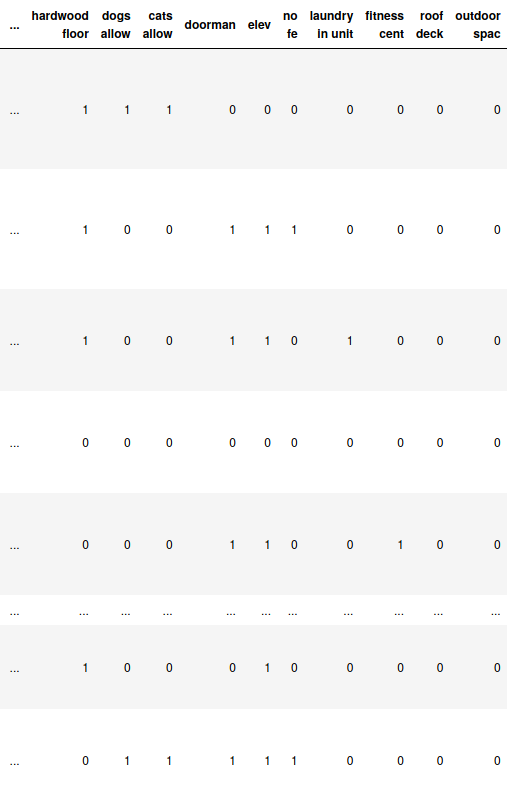
\includegraphics[width=7cm]{featureMarix.png}
    \caption{}
    \label{fig:galaxy}
\end{figure}



\\ For 'Description' (Figure 12):
\begin{itemize}
  \item removing the stop words, cleaning the text list, dropping punctuation, spaces and other irrelevant symbols;
  \item Stemming each description, as a word (using a build-in PorterStemmer);
  \item Analyzing and selecting the top words in {\bf B-gram} with high frequency as extracted features;
  \item concluding each extracted feature into individual columns, as binary values, to indicate which specific feature is present to each rental record. (ie. stainless steel', 'steel applianc', 'new york' and etc). Currently, every feature has been covered in a new column, which might be further discussed whether to keep or not.
\end{itemize}


\begin{figure}[h!]
    \centering
    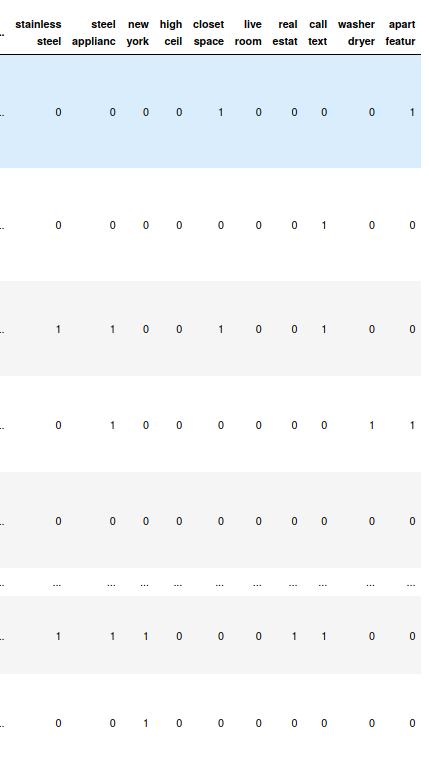
\includegraphics[width=7cm]{bgram.png}
    \caption{}
    \label{fig:galaxy}
\end{figure}



\end{document}
